\chapter{Discussion}

This chapter shows the results obtained during the evaluation and the tests we made to ensure the effectiveness of our models. 

\section{Testing flow?}

We write a function to execute different tests using different classificators and hyperparameters. 

As mentioned in Section \ref{sec:cv}, we used the \texttt{StratifiedKFold} class from \textit{Scikit-learn} to cross-validate our tests. This class has a method \texttt{split} that, given the train and test subsets, it returns a range of indexes to select only a portion of the dataset, as shown in Figure \ref{fig:stratified}.  At each fold, different parts of the dataset are chosen as a test subset, but summing the test subset in all the folds, we would obtain the entire dataset. Therefor we create two arrays where, at each fold, we append the predictions made by the classification model and the ones expected. At the end of the cross-validation algorithm, we use the \textit{Scikit-learn} functions \texttt{classification\_report}, \texttt{confusion\_matrix}, and \texttt{accuracy\_score}, with the complete arrays of predictions and expected values, to obtain the metrics needed to evaluate the model.

We chose $k = 10$ because, as shown in literature [cita quaclouno], it's the best value between performances and execution time. 
We set the \texttt{StratifiedKFold} option \texttt{shuffle} to true, so every time the cross-validation algorithm samples different binaries at each fold, avoiding that classification model focuses only on a very good or lousy subset of the dataset. Furthermore, we repeat each test 5 times, and then we average the results obtained.

For \texttt{RandomForest} and \texttt{XGBoost} models, we found that 300 trees are sufficient to get great results.

\section{Features selection}
In Section \ref{sec:feat_sel}, we presented different methods for feature selection. In this section, we analyze and compare them to find the best subset of features to represent APT malware.

\subsection{Scaling dataset}
The first step for selecting features is to scale the dataset. It is essential because, in our case, we have features with very different scales and contain some outliers. These two aspects can decrease the predictive performance of the classification model. We chose the \texttt{MaxAbsScaler} from \textit{scikit-learn} because it fits our needs. The scaler does not shift or center the data, and it does not destroy the sparsity of the features. For each feature, the algorithm calculates the maximum value and scales all the features in the column, such that the maximum value is equal to 1.0. All the features will be in the range of 0 and 1.0, but they maintain their variance.

\subsection{Remove low variance}
The second step is to visualize the variance of the dataset. We calculated with the std function on axis 0, and we visualize them with matplotlib. Figure \ref{fig:var_all} shows the variance of the entire dataset. As we can see, some features have zero variance, and this means that they are constant over all the samples. Thus they are not useful for classification.

\begin{figure}[!h]
	\centering
	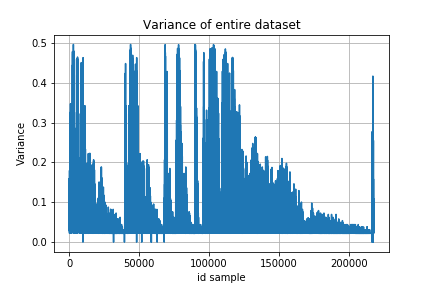
\includegraphics[width=0.6\columnwidth]{variance-all.png}
	\caption{Variance of features in the entire dataset}
	\label{fig:var_all}
\end{figure}

To remove them we use \texttt{VarianceThreshold} class that removes all low-variance features. Is it possible to set a threshold, if a feature variance is below the threshold, then it is removed. By default, the class removes all zero-variance features. This method removes \textbf{32} features from our dataset.

\subsection{Filter methods}

Filter methods works by selecting the best features based on a ranking function. Scikit-learn offers various scoring functions, such as \textit{chi2, f\_classif, mutual\_info\_classif}. To choose the best $k$ features scikit-learn has two classes:
\begin{itemize}
	\item \texttt{SelectKBest: }removes all but the highest $k$ scoring features.
	\item \texttt{SelectPercentile} removes all but a user-specified highest scoring percentage of features.
\end{itemize} 
We use \texttt{SelectPercentile} to perform some tests with different percentages and compared the results. 
We select respectivly the 25\%, 15\%, and 10\% of the functions \texttt{chi2, fclassif, and mutual\_info} and summarized them in Figures \ref{fig:ranking} and Tables \ref{tab:rank}. The column \textit{time} in Tables \ref{tab:rank} refers to the time elapsed during the feature selection, not during the classification algorithm to test the performances.

\begin{figure}[]
	\centering
	\begin{subfigure}[t]{0.48\textwidth}
		\centering
		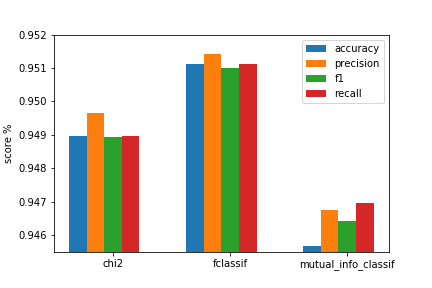
\includegraphics[width=\linewidth]{univariance25.png}
		\caption{Ranking functions score with 25\%}\label{fig:ranking25}		
	\end{subfigure}
	\begin{subfigure}[t]{0.48\textwidth}
		\centering
		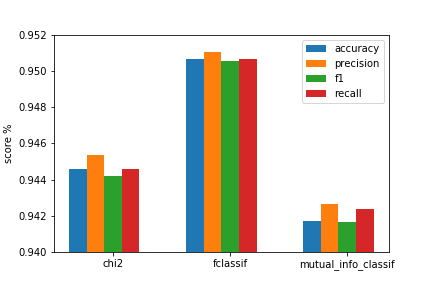
\includegraphics[width=\linewidth]{univariance15.png}
		\caption{Ranking functions score with 15\%}\label{fig:ranking15}
	\end{subfigure}\\
	\begin{subfigure}[t]{0.48\textwidth}
		\centering
		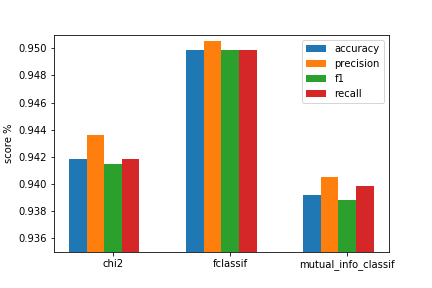
\includegraphics[width=\linewidth]{univariance10.png}
		\caption{Ranking functions score with 10\%}\label{fig:ranking10}
	\end{subfigure}
	\caption{Comparison of metrics score for different ranking functions with different percentages selected}\label{fig:ranking}
\end{figure}

As we can see from results the \texttt{f\_classif} is the one who perform the best, even if it takes a little more time than \texttt{chi2}, . On the contrary, \texttt{mutual\_info\_fclassif} is the slower, it takes half a day to calculate the mutuals information of the features, and it is also the worst in terms of performance.

However, as we reduce the percentage of features the performances degrade too. The best percentage is the 25\%, but it keeps over 50000 features, that are not good for our purpose. The classification time, instead, is acceptable, it varies from 58s for 25\% features, to 41s for 10\% features. 
We cannot rely only on filter methods because they would not shrink our dataset as we intended. So we tried other methods for features selection provided by \textit{scikit-learn}.




\begin{table}[]

	\caption{Comparison of metrics score for different ranking functions with different percentages 	\label{tab:rank}}
	\begin{subtable}{\linewidth}
	\centering
	\caption{Summary of ranking functions selecting the 25\% of the best features}
	\label{tab:rank_function}
	\begin{tabular}{llll}
		\toprule
		\textbf{Metrics}  & \textbf{chi2} & \textbf{fclassif }& \textbf{mutual\_info} \\
		\midrule
		\texttt{Time} & 7.60s & 246.05s & 43217.97s\\
		
		\texttt{Accuracy} & 94.90\% &  95.11\% &  94.57\% \\
		\texttt{Precision}  & 94.96\% & 95.14\% &   94.67\%   \\ 
		\texttt{Recall} & 94.90\%  &   95.11\%  & 94.70\% \\ 
		\texttt{F1-score}  &   94.89\%   & 95.10\% &    94.64\%      \\ 
		\bottomrule
	\end{tabular}
	\end{subtable}

	\begin{subtable}{\linewidth}
	\centering
	\caption{Summary of ranking functions selecting the 15\% of the best features}
	\label{tab:rank_function15}
	\begin{tabular}{llll}
		\toprule
		\textbf{Metrics}  & \textbf{chi2} & \textbf{fclassif }& \textbf{mutual\_info} \\
		\midrule
		\texttt{Time} & 7.60s & 246.05s & 43217.97s\\
		
		\texttt{Accuracy} & 94.46\% &  95.06\% &  94.17\% \\
		\texttt{Precision}  & 94.54\% & 95.1\% &   94.27\%   \\ 
		\texttt{Recall} & 94.46\%  &   95.06\%  & 94.24\% \\ 
		\texttt{F1-score}  &   94.42\%   & 95.06\% &    94.17\%      \\ 
		\bottomrule
	\end{tabular}
	\end{subtable}
\begin{subtable}{\linewidth}
	\centering
	\caption{Summary of ranking functions selecting the 10\% of the best features}
	\label{tab:rank_function10}
	\begin{tabular}{llll}
		\toprule
		\textbf{Metrics}  & \textbf{chi2} & \textbf{fclassif }& \textbf{mutual\_info} \\
		\midrule
		\texttt{Time} & 7.60s & 246.05s & 43217.97s\\
		
		\texttt{Accuracy} & 94.19\% &  94.99\% &  93.92\% \\
		\texttt{Precision}  & 94.36\% & 95.05\% &   94.05\%   \\ 
		\texttt{Recall} & 94.19\%  &   94.99\%  & 93.99\% \\ 
		\texttt{F1-score}  &   94.15\%   & 94.98\% &    93.89\%      \\ 
		\bottomrule
	\end{tabular}
\end{subtable}
	
	
\end{table}


\subsection{Embedded Methods}

Embedded methods use models that have build-in feature selection methods. \texttt{RandomForestClassifier} has a field \texttt{feature\_importances} to rank all the features from best to worst. In particular \textit{scikit-learn} provides a \texttt{SelectFromModel} class, that using a classifier that has a build-in feature importance method, select the best features based on the model. It is possible to set a \texttt{max\_features} parameter, to limit the number of selected features.

However, the \texttt{SelectFromModel} algorithm chooses 12781 features in just 18s. Even with \texttt{max\_features} set to 21781 (the 10\% of the entire dataset), the algorithm still chooses only the 12781 features. Comparing the performances with the filter methods presented before we find that \texttt{SelectFromModel} is more accurate and the fastest in classification because there are less features. Based on those tests we prefer to discard filter methods and keep using \texttt{SelectFromModel}.

\begin{figure}[]
	\centering
	\begin{subfigure}[t]{0.48\textwidth}
		\centering
		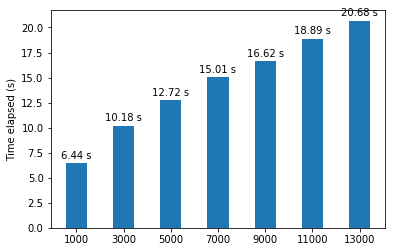
\includegraphics[width=\linewidth]{selmodel-time.png}
		\caption{Time comparison}\label{fig:model-time}		
	\end{subfigure}
	\begin{subfigure}[t]{0.48\textwidth}
		\centering
		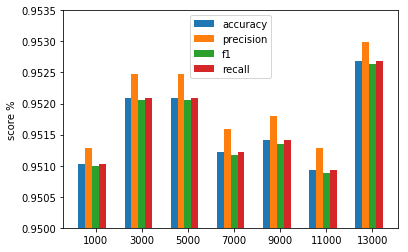
\includegraphics[width=\linewidth]{selmodel-metrics.png}
		\caption{Metrics comparison}\label{fig:model-metrics}
	\end{subfigure}
	\caption{Comparison of time and metrics score with different number of features selected using \texttt{SelectFromModel}}\label{fig:model}
\end{figure}


We run various tests with different numbers of \texttt{max	features} to compare the results. The tests are shown in Figure \ref{fig:model}. Figure \ref{fig:model-time} shows how the time varies related to the number of features selected.

As we can see from Figure \ref{fig:model-metrics} there is no big difference in the tests made between \textit{accuracy, precision,recall, or f1-score}. For example, the maximum difference in accuracy is just 0.0016s. This happens because \texttt{RandomForestClassifier} already performs features selection using \texttt{feature\_importances} during the training phase. Since the time is dependent to the number of features, we choose to balance the performances and the execution time, thus we select the best 3000 features.
